%%%%%%%%%%%%%%%%%%%%%%%%%%%%%%%%%%%%%%%%%%%%%%%%%%%%%%%%%%%%%%%%%%%%%%%%%%%%%%%%
\chapter*{Основная часть} % Заголовок
\addcontentsline{toc}{chapter}{Основная часть} % Добавить в оглавление
\refstepcounter{chapter} % Счётчик

%%%%%%%%%%%%%%%%%%%%%%%%%%%%%%%%%%%%%%%%%%%%%%%%%%%%%%%%%%%%%%%%%%%%%%%%%%%%%%%%
%%%%%%%%%%%%%%%%%%%%%%%%%%%%%%%%%%%%%%%%%%%%%%%%%%%%%%%%%%%%%%%%%%%%%%%%%%%%%%%%
\section{Метод полностью параллельной разностной эволюции} \label{s1}

Метод ППРЭ успешно применялся в~различных задачах~\cite{bib3,bib4}.
Совершенствование методов минимизации для нахождения параметров генных 
регуляторных сетей требует наличия набора тестов для оценки новых алгоритмов 
и~реализаций и~сравнения с~предшествующими. 

В самом общем смысле класс рассматриваемых задач можно назвать задачами 
поиска глобального минимума некоторого функционала качества (или функции). 
Способов решения таких задач достаточно много. В работе рассматривается 
модификация стохастического итерационного метода разностной эволюции (РЭ). 
Идея метода РЭ, предложенного Р.~Сторном~\cite{bib1}, заключается в 
моделировании популяции индивидуумов (а точнее, векторов их определяющих). 
Популяция меняется от поколения к поколению, при этом индивидуумы скрещиваются 
и мутируют. 

Метод РЭ имеет набор управляющих параметров (например, размер популяции 
или количество старейших индивидуумов, заменяемых на новые), от которых сильно 
зависит скорость работы и сходимость. Возраст индивидуума — количество итераций,
которые он существует. В~\cite{bibZaharie} была предложена адаптивная схема 
выбора управляющих параметров метода РЭ. В работе~\cite{bibTM} введено 
тригонометрическое преобразование (мутация) вектора-индивидуума, зависящее от 
функционала качества. 

В данной работе рассматривается метод ППРЭ~\cite{bib2,bib5}. Спустя определённое
количество итераций $es\_lambda$ самых старых индивидуумов заменяется 
на~$es\_lambda$ самых «лучших».

\clearpage
%%%%%%%%%%%%%%%%%%%%%%%%%%%%%%%%%%%%%%%%%%%%%%%%%%%%%%%%%%%%%%%%%%%%%%%%%%%%%%%%
%%%%%%%%%%%%%%%%%%%%%%%%%%%%%%%%%%%%%%%%%%%%%%%%%%%%%%%%%%%%%%%%%%%%%%%%%%%%%%%%
\section{Экспериментальные данные (DREAM)} \label{s2}

Проект DREAM предоставляет унифицированные экспериментальные данные для 
тестирования алгоритмов. Каждое «испытание» — некая формализованная задача,
которую предлагается решить независимым группам исследователей. 
Лучшие решения и результаты публикуются. \cite{bib6}. 

В рамках этой работы требуется подобрать близкие к оптимальным значения 
параметров ППРЭ, используя в качестве тестовых задач результаты DREAM6.

%%%%%%%%%%%%%%%%%%%%%%%%%%%%%%%%%%%%%%%%%%%%%%%%%%%%%%%%%%%%%%%%%%%%%%%%%%%%%%%%
\subsection{Постановка задачи} \label{s2_1}

Задача принадлежит области обратной инженерии генных регуляторных сетей. 
Предполагается, что топология генной сети уже определена с достаточным уровнем 
правдоподобия, и теперь требуется охарактеризовать параметры (кинетику) 
этой сети.

Здесь есть два ключевых аспекта, которые требуют внимания: задача оценки 
параметров модели по данной структуре модели, а так же задача проектирования 
наиболее информативных экспериментов для получения неизвестных параметров. 

Итак, даны структуры трёх генных регуляторных сетей, от участников требуется 
разработать и/или применять методы оптимизации, чтобы точно оценить 
параметры моделей, а так же прогнозировать результаты возмущений в этих моделях.

Эти две задачи и являются областью исследования DREAM6. Однако, для тестирования
ППРЭ потребуется рассмотреть лишь первую задачу.

%%%%%%%%%%%%%%%%%%%%%%%%%%%%%%%%%%%%%%%%%%%%%%%%%%%%%%%%%%%%%%%%%%%%%%%%%%%%%%%%
\subsection{Модели генных сетей: Представление данных} \label{s2_2}

Полные структуры генных сетей представлены в формате sbml, tic, и в графическом 
формате. Пример такого представления для первой генной сети приведён на 
рисунке~\ref{img:GrnImage}.

\begin{figure}[h]
  \center{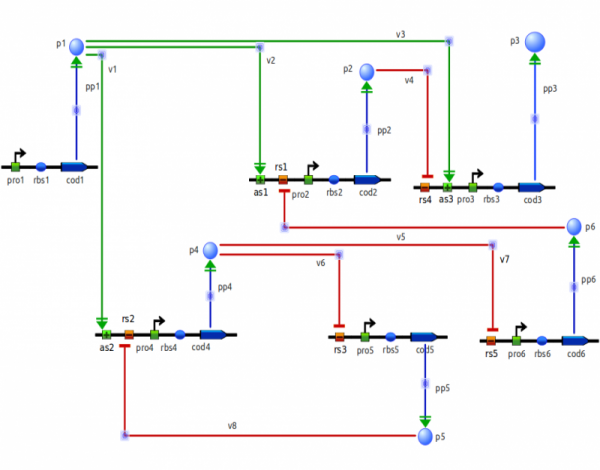
\includegraphics[width=14cm]{model1-600x470.png}}
  \caption{Пример графического представления для первой генной сети}
  \label{img:GrnImage}
\end{figure}

\begin{figure}[h]
  \begin{minipage}[h]{0.34\linewidth}
    \center{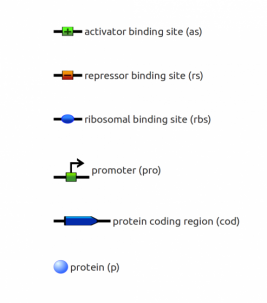
\includegraphics[height=8cm]{diagram_key-267x303.png}}
    \caption{Аннотация к графическому представлению}
    \label{img:GrnImageDesc}
  \end{minipage}
  \hfill
  \begin{minipage}[h]{0.64\linewidth}
    \center{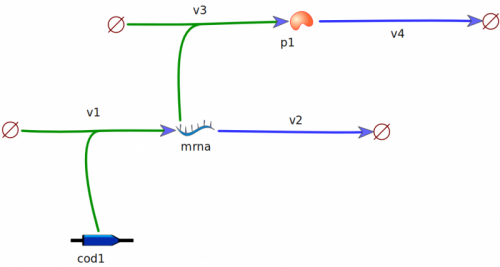
\includegraphics[height=6cm]{protein_production_subfigure-500x267.png}}
    \caption{Транскрипция и трансляция, не показанные на схеме генной сети}
    \label{img:GrnImageTT}
  \end{minipage}
\end{figure}

Для каждой сети предоставляется файл (.m) с описанием модели в 
синтаксисе MATLAB. Все переменные помечены в соответствии с их типом. 
Например, переменные, означающие концентрацию белка, помечены как 
$p1$,~$p2$,~...~$p6$. 

Значения каждого символа в генной сети подробно 
объясняются в легенде (рис.~\ref{img:GrnImageDesc}). В скобках перечислены 
префиксы к переменным модели. Линии, соединяющие кодирующую белок 
последовательность с белком, обозначены префиксом «pp». Генерация белка состоит 
из двух логических частей: транскрипция и трансляция. Для простоты эти два 
этапа, изображённые на схеме~\ref{img:GrnImageTT}, не показаны в диаграмме 
генной сети. 

Имена переменных для мРНК, для результата транскрипции кодирующей 
последовательности имеют соответствующий префикс «pp». Например, мРНК, 
соответствующая $pp3$ будет именована как $pp3\_mrna$.

%%%%%%%%%%%%%%%%%%%%%%%%%%%%%%%%%%%%%%%%%%%%%%%%%%%%%%%%%%%%%%%%%%%%%%%%%%%%%%%%
\subsection{Параметры генных сетей} \label{s2_3}

Генная сеть характеризуется топологией (структурой), о которой говорилось выше, 
и набором параметров — скорость трансляции, транскрипции, и параметров, 
отвечающих за сайты связывания рибосом. Если все эти параметры и начальные 
данные (начальные концентрации мРНК) определены, рассматривается поведение 
генной сети на фиксированном интервале времени. Под поведением здесь имеется 
ввиду динамика изменения концентраций мРНК и белка каждого типа.

Таким образом, каждая генная сеть с заданными параметрами порождает матрицу, 
содержащую набор концентраций для фиксированных моментов времени. В DREAM6 от
участников требуется решить обратную задачу: по данной матрице концентраций 
(пример матрицы~\ref{mRNAtable}) предоставить набор параметров сети.

%%%%%%%%%%%%%%%%%%%%%%%%%%%%%%%%%%%%%%%%%%%%%%%%%%%%%%%%%%%%%%%%%%%%%%%%%%%%%%%%
\subsection{Начальные данные и возмущения} \label{s2_4}

Наборы данных, которые предоставляются в качестве входных для оценки параметров,
были сформированы искусственно, путем моделирования, с учётом различных 
возмущений (зашумлений) в генной сети — делеции гена, мРНК нокдаун и изменение 
активности сайтов связывания рибосом. 

Оговорено, что во всех случаях возмущения могут затрагивать только один ген. 
Удаление гена приводит к полной ликвидации как мРНК, так и белка целевого гена. 
В случае миРНК, мРНК деградирует (фиксированное уменьшение в 5 раз), что 
приводит к уменьшению как мРНК, так и концентрации соответствующего белка.

\begin{table}[h]
  \centering
    \begin{tabular}{l|llllll}
        0.0	  & 0.0    & 0.0   & 0.041  & 0.16  & 0.189  & 0.048 \\
        2.0	  & 2.754  & 4.01  & 4.531  & 0.30  & 0.221  & 0.006 \\
        4.0	  & 2.958  & 2.96  & 0.911  & 0.06  & 0.522  & 0.39  \\
        6.0	  & 4.058  & 2.18  & 0.457  & 0.07  & 1.609  & 1.266 \\
        8.0	  & 3.41   & 1.06  & 0.649  & 0.08  & 2.627  & 2.253 \\
        10.0  & 3.459  & 0.68  & 4.398  & 0.07  & 2.979  & 3.811 \\
        12.0  & 2.453  & 0.67  & 6.734  & 0.27  & 2.618  & 2.983 \\
        14.0  & 1.234  & 0.43  & 5.971  & 0.02  & 2.443  & 3.025 \\
        16.0  & 2.385  & 0.43  & 4.606  & 0.0   & 1.821  & 2.823 \\
        18.0  & 3.691  & 0.52  & 5.827  & 0.0   & 3.444  & 2.386 \\
        20.0  & 3.252  & 0.4   & 8.947  & 0.0   & 4.358  & 3.666 
    \end{tabular}
  \caption{Пример таблицы концентраций мРНК для первой генной сети}
  \label{mRNAtable}
\end{table}

\clearpage
%%%%%%%%%%%%%%%%%%%%%%%%%%%%%%%%%%%%%%%%%%%%%%%%%%%%%%%%%%%%%%%%%%%%%%%%%%%%%%%%
%%%%%%%%%%%%%%%%%%%%%%%%%%%%%%%%%%%%%%%%%%%%%%%%%%%%%%%%%%%%%%%%%%%%%%%%%%%%%%%%
\section{Численные эксперименты} \label{s3}

%%%%%%%%%%%%%%%%%%%%%%%%%%%%%%%%%%%%%%%%%%%%%%%%%%%%%%%%%%%%%%%%%%%%%%%%%%%%%%%%
\subsection{Постановка задачи в терминах метода ППРЭ} \label{s3_1}

Метод ППРЭ ищет минимум функционала качества по списку параметров. Параметры — 
неопределённые параметры генной сети, о которых говорилось в предыдущей главе. 

За функционал качества выбирается расстояние между заранее определённой матрицей 
концентраций $W$ (см.~\ref{s2_3}) и матрицей концентраций, полученной с текущими 
параметрами. При этом расстояние понимается как сумма квадратов поэлементных 
разностей двух матриц. 

Как уже было сказано, в качестве оценки работы ППРЭ используются две 
характеристики: 
\begin{enumerate}
	\item Расстояние между известной и полученной матрицами концентраций. Т.е. 
	функционал качества.
	\item Расстояние между известными и полученными параметрами
\end{enumerate}

Более формально: генная сеть, при выборе вектора параметров $p$ и задании
вектора начальных условий $e$ порождает дифференциальное уравнение $ODE(p,e)$. В 
силу однозначности начальных данных, решение этого уравнения единственно. 
Решение — динамика изменений концентраций мРНК и соответствующих им белков. При
фиксированном интервале времени и разбиении решение есть матрица концентраций 
$M^{(p,e)}$.

\[ (p,e) \rightarrow ODE(p,e) \rightarrow M^{(p,e)} \]

Так как вектор начальных условий $e$ неизменен и определён, конструкция 
упрощается:

\[ p \rightarrow ODE(p) \rightarrow M^p \]

Функционал качества для метода ППРЭ есть Евклидово расстояние между матрицами 
концентраций, а $\rho$ есть:

\[ \rho(p,p^*) = \frac{1}{N} \sum\limits_{i = 1}^{N} ln(p_i/p^*_i)^2 \]

Где N — размерность векторов $p$ (текущие параметры) и $p^*$ (известные 
параметры). Теперь каждый вектор параметров $p$ порождает два числа (две 
характеристики, о~которых говорилось выше):

\[ 
p \rightarrow ODE(p) \rightarrow M^p 
\rightarrow \{ \sum\limits_{i,j}(M_{i,j}^p - W_{i,j})^2 , \rho(p,p^*) \}
\]

%%%%%%%%%%%%%%%%%%%%%%%%%%%%%%%%%%%%%%%%%%%%%%%%%%%%%%%%%%%%%%%%%%%%%%%%%%%%%%%%
\subsection{Прогонка управляющих параметров ППРЭ} \label{s3_2}

В качестве критерия остановки было выбрано время, прошедшее с момента начала 
работы. Для каждого запуска выделялось 900 секунд. 

Для всех трёх моделей был зафиксирован параметр $population\_size = 150$ 
($p.size$) и~варьировалось $es\_lambda = 2,15,45$ ($es\_l.$). Всего было 
проведено 12 запусков для каждой модели. 

\begin{table}[h]
\centering
\def\arraystretch{1.5} % отступы
\begin{tabular}{|l|l|llllll|}
\hline % ================================================== %
  \multirow{2}{*}{p.size} & 
  \multirow{2}{*}{es\_l.} & 
  \multicolumn{2}{c|}{Модель 1} & 
  \multicolumn{2}{c|}{Модель 2} & 
  \multicolumn{2}{c|}{Модель 3} \\ \cline{3-8} 
  & & 
  \multicolumn{1}{c|}{Среднее} & 
  \multicolumn{1}{c|}{Мин.} & 
  \multicolumn{1}{c|}{Среднее} & 
  \multicolumn{1}{c|}{Мин.} & 
  \multicolumn{1}{c|}{Среднее} & 
  \multicolumn{1}{c|}{Мин.} \\ 

\hline % ================================================== %
\multirow{3}{*}{150} 
 & 2  & 49.3667 & 25.4139 & 22.8473 & 12.1157 & 48.6207 & 35.7457 \\ \cline{2-2}
 & 15 & 44.0293 & 30.755  & 25.8365 & 12.1114 & 49.8181 & 30.1344 \\ \cline{2-2}
 & 45 & 44.3788 & 24.9287 & 24.1793 & 15.0964 & 44.8327 & 34.6884 \\ 

\hline % ================================================== %
\multicolumn{2}{|l|}{$\Sigma$} & 
\multicolumn{2}{l|}{46.51614} & 
\multicolumn{2}{l|}{20.43136} & 
\multicolumn{2}{l|}{55.38312} \\ 

\hline % ================================================== %
\end{tabular}
\end{table}

Здесь $\Sigma$ — значение функционала качества для известных параметров $p^*$.
Динамика изменений $\Sigma$ отражена на графиках:
% \[ \sum\limits_{i,j}(M_{i,j}^{p^*} - W_{i,j})^2 \]

\begin{figure}[h]
  \center{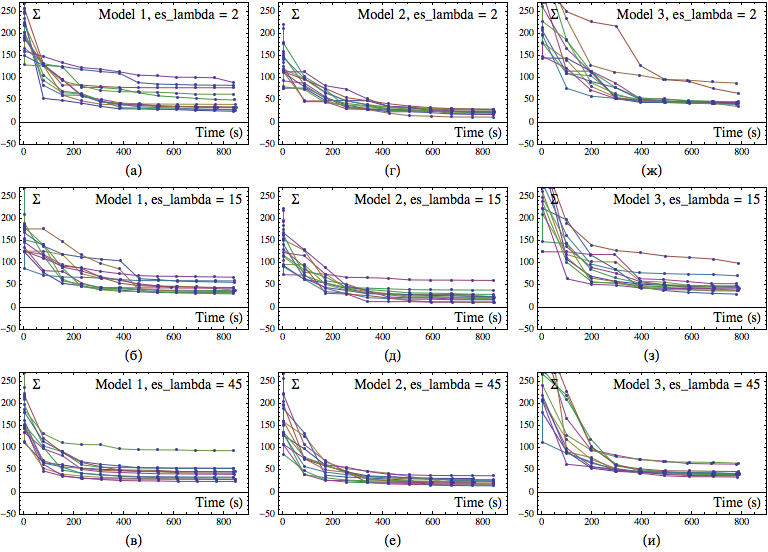
\includegraphics[width=17cm]{p150}}
  \caption{Динамика изменения $\Sigma$. Три модели. 12 независимых запусков. 
  $population\_size = 150$. Модели генных сетей (1,~2,~3) по столбцам, 
  по вертикали: $es\_lambda = 2, 15, 45$. }
  \label{img:p150}
\end{figure}

Из графиков и таблицы очевидно, что в среднем значение минимизируемого 
функционала сходится своему минимальному значению. Кроме того, всегда находился 
набор параметров (вектор $p$, значение $\Sigma$ для которого меньше эталонного).

Рассмотрм изменение расстояния $\rho$ между известными параметрами генной сети 
(предоставленными) и параметрами, найденными методом ППРЭ.

\begin{figure}[h]
  \center{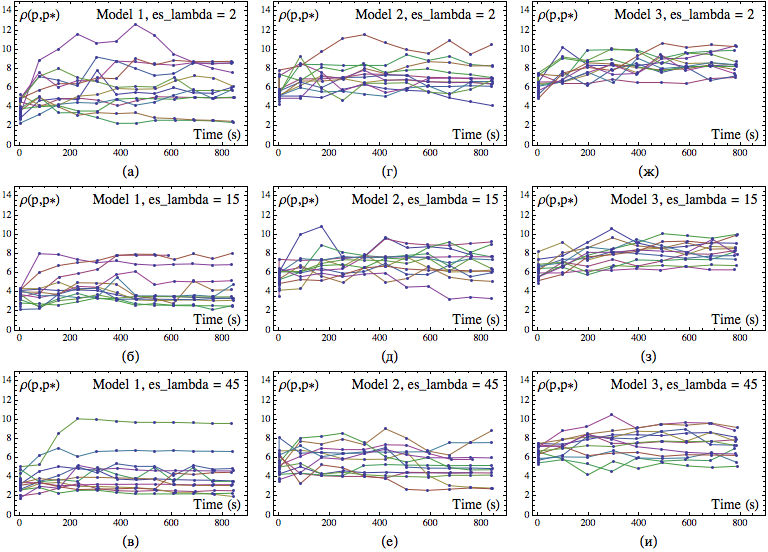
\includegraphics[width=17cm]{p150e}}
  \caption{Динамика изменения $\rho$. Три модели. 12 независимых запусков. 
  $population\_size = 150$. Модели генных сетей (1,~2,~3) по столбцам, 
  по вертикали: $es\_lambda = 2, 15, 45$. }
  \label{img:p150}
\end{figure}

Из графиков видно, что ППРЭ находит не тот вектор, который представлен в 
качестве ответа. Надо полагать, что это происходит из-за большого количества 
параметров ДУ.

Посмотрим, что из себя представляют таблицы концентраций при использовании 
вектора параметров $p$ и $p^*$. Однако, для наглядности рассмотрим не сами 
таблицы $M^p$, а их отличие (разности) от таблицы $W$, т.е. $M - W$:

% На рисунках ниже изображены сами таблицы и их графики. 
% Во всех таблицах строка $i$ соответствует моменту времени $(i - 1) * 0.2$ с., 
% столбец $j$ есть модуль разности концентраций мРНК с номером $j$

\begin{table}[h]
  \centering
  \begin{tabular}{|llllll|}
\color[HTML]{909090}0. & \color[HTML]{909090}0. & \color[HTML]{808080}0.041 & \color[HTML]{606060}0.166 & \color[HTML]{505050}0.189 & \color[HTML]{808080}0.048 \\ 
\color[HTML]{606060}0.16 & \color[HTML]{707070}0.093 & \color[HTML]{000000}0.94 & \color[HTML]{606060}0.15 & \color[HTML]{909090}0.02 & \color[HTML]{404040}0.235 \\ 
\color[HTML]{909090}0.013 & \color[HTML]{808080}0.035 & \color[HTML]{707070}0.103 & \color[HTML]{808080}0.035 & \color[HTML]{000000}0.563 & \color[HTML]{000000}0.695 \\ 
\color[HTML]{000000}1.065 & \color[HTML]{000000}0.874 & \color[HTML]{000000}1.204 & \color[HTML]{808080}0.074 & \color[HTML]{000000}0.852 & \color[HTML]{000000}1.195 \\ 
\color[HTML]{101010}0.411 & \color[HTML]{202020}0.366 & \color[HTML]{000000}3.889 & \color[HTML]{707070}0.087 & \color[HTML]{303030}0.286 & \color[HTML]{000000}0.66 \\ 
\color[HTML]{000000}0.459 & \color[HTML]{606060}0.142 & \color[HTML]{000000}1.301 & \color[HTML]{808080}0.073 & \color[HTML]{909090}0.009 & \color[HTML]{000000}0.823 \\ 
\color[HTML]{000000}0.547 & \color[HTML]{606060}0.173 & \color[HTML]{000000}0.807 & \color[HTML]{303030}0.277 & \color[HTML]{101010}0.38 & \color[HTML]{909090}0.015 \\ 
\color[HTML]{000000}1.766 & \color[HTML]{808080}0.067 & \color[HTML]{909090}0.003 & \color[HTML]{909090}0.024 & \color[HTML]{000000}0.557 & \color[HTML]{909090}0.025 \\ 
\color[HTML]{000000}0.615 & \color[HTML]{808080}0.065 & \color[HTML]{000000}1.369 & \color[HTML]{909090}0. & \color[HTML]{000000}1.179 & \color[HTML]{505050}0.177 \\ 
\color[HTML]{000000}0.691 & \color[HTML]{808080}0.027 & \color[HTML]{606060}0.15 & \color[HTML]{909090}0. & \color[HTML]{000000}0.444 & \color[HTML]{000000}0.614 \\ 
\color[HTML]{404040}0.252 & \color[HTML]{707070}0.096 & \color[HTML]{000000}2.97 & \color[HTML]{909090}0. & \color[HTML]{000000}1.358 & \color[HTML]{000000}0.666
\end{tabular}

  \caption{Модель 1. Таблица концентраций получена параметрами $p^*$, 
  предлагаемыми DREAM6 в качестве ответа. $|W - M^{p^*}|$}
  \label{m1p2}
\end{table}
\begin{table}[h]
  \centering
  \begin{tabular}{|llllll|}
\color[HTML]{909090}0. & \color[HTML]{909090}0. & \color[HTML]{808080}0.041 & \color[HTML]{606060}0.166 & \color[HTML]{505050}0.189 & \color[HTML]{808080}0.048 \\ 
\color[HTML]{606060}0.163 & \color[HTML]{000000}1.119 & \color[HTML]{404040}0.258 & \color[HTML]{606060}0.151 & \color[HTML]{505050}0.221 & \color[HTML]{808080}0.028 \\ 
\color[HTML]{909090}0.017 & \color[HTML]{101010}0.391 & \color[HTML]{707070}0.117 & \color[HTML]{606060}0.127 & \color[HTML]{000000}0.521 & \color[HTML]{909090}0. \\ 
\color[HTML]{000000}1.069 & \color[HTML]{404040}0.258 & \color[HTML]{303030}0.275 & \color[HTML]{909090}0.011 & \color[HTML]{303030}0.307 & \color[HTML]{303030}0.315 \\ 
\color[HTML]{101010}0.415 & \color[HTML]{505050}0.203 & \color[HTML]{505050}0.183 & \color[HTML]{707070}0.075 & \color[HTML]{707070}0.079 & \color[HTML]{404040}0.256 \\ 
\color[HTML]{000000}0.463 & \color[HTML]{707070}0.103 & \color[HTML]{505050}0.193 & \color[HTML]{808080}0.071 & \color[HTML]{606060}0.166 & \color[HTML]{000000}1.009 \\ 
\color[HTML]{000000}0.543 & \color[HTML]{808080}0.034 & \color[HTML]{000000}0.583 & \color[HTML]{303030}0.277 & \color[HTML]{505050}0.209 & \color[HTML]{707070}0.122 \\ 
\color[HTML]{000000}1.762 & \color[HTML]{505050}0.177 & \color[HTML]{000000}0.452 & \color[HTML]{909090}0.024 & \color[HTML]{101010}0.386 & \color[HTML]{606060}0.155 \\ 
\color[HTML]{000000}0.611 & \color[HTML]{606060}0.168 & \color[HTML]{000000}1.86 & \color[HTML]{909090}0. & \color[HTML]{000000}1.009 & \color[HTML]{808080}0.049 \\ 
\color[HTML]{000000}0.695 & \color[HTML]{707070}0.075 & \color[HTML]{000000}0.647 & \color[HTML]{909090}0. & \color[HTML]{000000}0.614 & \color[HTML]{000000}0.486 \\ 
\color[HTML]{404040}0.256 & \color[HTML]{505050}0.197 & \color[HTML]{000000}2.472 & \color[HTML]{909090}0. & \color[HTML]{000000}1.528 & \color[HTML]{000000}0.794
\end{tabular}

  \caption{Модель 1. Таблица концентраций получена подбором параметров 
  $p_{min}$ методом ППРЭ. $|W - M^{p_{min}}|$}
  \label{m1p3}
\end{table}
\begin{figure}[h]
  \begin{minipage}[h]{0.5\linewidth}
    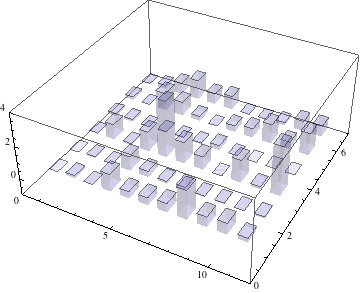
\includegraphics[width=8cm]{tables1f2}
    \caption{График таблицы \ref{m1p2} для $p^*$}
  \end{minipage}
  \hfill
  \begin{minipage}[h]{0.5\linewidth}
    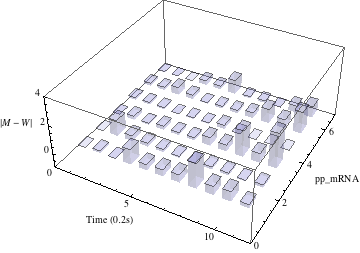
\includegraphics[width=8cm]{tables1f3}
    \caption{График таблицы \ref{m1p3} для $p_{min}$}
  \end{minipage}
\end{figure}


\begin{table}[h]
  \centering
  \begin{tabular}{|lllllll|}
\color[HTML]{909090}0. & \color[HTML]{909090}0. & \color[HTML]{808080}0.044 & \color[HTML]{909090}0. & \color[HTML]{909090}0. & \color[HTML]{707070}0.114 & \color[HTML]{909090}0. \\ 
\color[HTML]{606060}0.132 & \color[HTML]{303030}0.319 & \color[HTML]{505050}0.177 & \color[HTML]{000000}0.896 & \color[HTML]{000000}0.504 & \color[HTML]{404040}0.252 & \color[HTML]{505050}0.219 \\ 
\color[HTML]{707070}0.102 & \color[HTML]{505050}0.187 & \color[HTML]{303030}0.303 & \color[HTML]{606060}0.143 & \color[HTML]{505050}0.176 & \color[HTML]{606060}0.173 & \color[HTML]{000000}1.235 \\ 
\color[HTML]{000000}0.441 & \color[HTML]{000000}1.121 & \color[HTML]{505050}0.2 & \color[HTML]{909090}0.013 & \color[HTML]{909090}0.01 & \color[HTML]{303030}0.288 & \color[HTML]{000000}1.467 \\ 
\color[HTML]{606060}0.152 & \color[HTML]{000000}1.236 & \color[HTML]{101010}0.413 & \color[HTML]{909090}0.003 & \color[HTML]{404040}0.256 & \color[HTML]{000000}1.086 & \color[HTML]{000000}0.444 \\ 
\color[HTML]{606060}0.142 & \color[HTML]{000000}0.434 & \color[HTML]{000000}0.428 & \color[HTML]{808080}0.059 & \color[HTML]{909090}0.011 & \color[HTML]{000000}1.122 & \color[HTML]{707070}0.085 \\ 
\color[HTML]{303030}0.3 & \color[HTML]{000000}0.722 & \color[HTML]{000000}0.979 & \color[HTML]{909090}0. & \color[HTML]{707070}0.119 & \color[HTML]{000000}1.893 & \color[HTML]{909090}0.006 \\ 
\color[HTML]{404040}0.233 & \color[HTML]{101010}0.39 & \color[HTML]{000000}0.739 & \color[HTML]{808080}0.063 & \color[HTML]{000000}0.593 & \color[HTML]{808080}0.052 & \color[HTML]{707070}0.117 \\ 
\color[HTML]{404040}0.251 & \color[HTML]{000000}0.648 & \color[HTML]{404040}0.236 & \color[HTML]{808080}0.063 & \color[HTML]{707070}0.103 & \color[HTML]{404040}0.262 & \color[HTML]{505050}0.203 \\ 
\color[HTML]{808080}0.071 & \color[HTML]{707070}0.097 & \color[HTML]{000000}0.487 & \color[HTML]{606060}0.166 & \color[HTML]{404040}0.264 & \color[HTML]{000000}0.574 & \color[HTML]{909090}0.013 \\ 
\color[HTML]{909090}0.006 & \color[HTML]{000000}0.574 & \color[HTML]{000000}0.886 & \color[HTML]{909090}0.024 & \color[HTML]{808080}0.067 & \color[HTML]{505050}0.213 & \color[HTML]{909090}0.
\end{tabular}

  \caption{Модель 2. Таблица концентраций получена параметрами $p^*$, 
  предлагаемыми DREAM6 в качестве ответа. $|W - M^{p^*}|$}
  \label{m2p2}
\end{table}
\begin{table}[h]
  \centering
  \begin{tabular}{|lllllll|}
\color[HTML]{909090}0. & \color[HTML]{909090}0. & \color[HTML]{808080}0.044 & \color[HTML]{909090}0. & \color[HTML]{909090}0. & \color[HTML]{707070}0.114 & \color[HTML]{909090}0. \\ 
\color[HTML]{808080}0.031 & \color[HTML]{101010}0.388 & \color[HTML]{606060}0.171 & \color[HTML]{000000}0.583 & \color[HTML]{808080}0.027 & \color[HTML]{000000}0.432 & \color[HTML]{404040}0.227 \\ 
\color[HTML]{303030}0.287 & \color[HTML]{000000}0.602 & \color[HTML]{101010}0.401 & \color[HTML]{000000}0.495 & \color[HTML]{505050}0.2 & \color[HTML]{404040}0.263 & \color[HTML]{000000}0.548 \\ 
\color[HTML]{000000}0.629 & \color[HTML]{000000}0.895 & \color[HTML]{000000}0.794 & \color[HTML]{909090}0.004 & \color[HTML]{808080}0.053 & \color[HTML]{606060}0.154 & \color[HTML]{909090}0.005 \\ 
\color[HTML]{808080}0.037 & \color[HTML]{000000}1.08 & \color[HTML]{707070}0.1 & \color[HTML]{808080}0.06 & \color[HTML]{303030}0.295 & \color[HTML]{000000}0.597 & \color[HTML]{303030}0.307 \\ 
\color[HTML]{808080}0.046 & \color[HTML]{000000}0.568 & \color[HTML]{808080}0.056 & \color[HTML]{707070}0.121 & \color[HTML]{808080}0.028 & \color[HTML]{000000}0.662 & \color[HTML]{808080}0.067 \\ 
\color[HTML]{707070}0.112 & \color[HTML]{000000}0.848 & \color[HTML]{000000}0.504 & \color[HTML]{808080}0.061 & \color[HTML]{707070}0.081 & \color[HTML]{000000}1.437 & \color[HTML]{909090}0.009 \\ 
\color[HTML]{808080}0.045 & \color[HTML]{404040}0.266 & \color[HTML]{404040}0.266 & \color[HTML]{909090}0.003 & \color[HTML]{000000}0.555 & \color[HTML]{000000}0.575 & \color[HTML]{707070}0.117 \\ 
\color[HTML]{808080}0.063 & \color[HTML]{000000}0.525 & \color[HTML]{404040}0.236 & \color[HTML]{909090}0.003 & \color[HTML]{808080}0.065 & \color[HTML]{404040}0.248 & \color[HTML]{505050}0.203 \\ 
\color[HTML]{404040}0.259 & \color[HTML]{808080}0.026 & \color[HTML]{909090}0.015 & \color[HTML]{404040}0.226 & \color[HTML]{303030}0.302 & \color[HTML]{808080}0.071 & \color[HTML]{909090}0.013 \\ 
\color[HTML]{505050}0.194 & \color[HTML]{000000}0.697 & \color[HTML]{101010}0.414 & \color[HTML]{808080}0.036 & \color[HTML]{808080}0.029 & \color[HTML]{000000}0.713 & \color[HTML]{909090}0.
\end{tabular}

  \caption{Модель 2. Таблица концентраций получена подбором параметров 
  $p_{min}$ методом ППРЭ. $|W - M^{p_{min}}|$}
  \label{m2p3}
\end{table}
\begin{figure}[h]
  \begin{minipage}[h]{0.5\linewidth}
    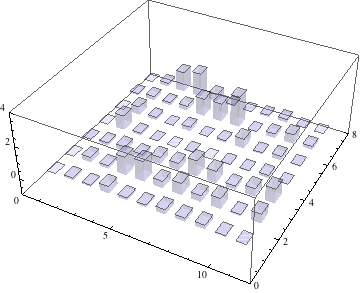
\includegraphics[width=8cm]{tables2f2}
    \caption{График таблицы \ref{m2p2} для $p^*$}
  \end{minipage}
  \hfill
  \begin{minipage}[h]{0.5\linewidth}
    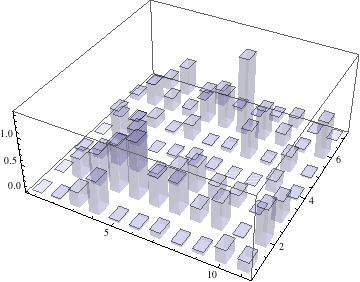
\includegraphics[width=8cm]{tables2f3}
    \caption{График таблицы \ref{m2p3} для $p_{min}$}
  \end{minipage}
\end{figure}


\begin{table}[h]
  \centering
  \begin{tabular}{|lllllllll|}
\color[HTML]{808080}0.072 & \color[HTML]{909090}0. & \color[HTML]{606060}0.127 & \color[HTML]{808080}0.074 & \color[HTML]{909090}0.011 & \color[HTML]{909090}0. & \color[HTML]{909090}0. & \color[HTML]{707070}0.08 & \color[HTML]{909090}0. \\ 
\color[HTML]{505050}0.19 & \color[HTML]{000000}1.026 & \color[HTML]{000000}0.53 & \color[HTML]{000000}0.882 & \color[HTML]{000000}0.636 & \color[HTML]{000000}0.892 & \color[HTML]{000000}1.003 & \color[HTML]{000000}1.472 & \color[HTML]{000000}1.741 \\ 
\color[HTML]{808080}0.052 & \color[HTML]{909090}0.021 & \color[HTML]{000000}3.475 & \color[HTML]{000000}3.462 & \color[HTML]{909090}0.015 & \color[HTML]{707070}0.117 & \color[HTML]{404040}0.258 & \color[HTML]{505050}0.219 & \color[HTML]{000000}0.581 \\ 
\color[HTML]{808080}0.058 & \color[HTML]{909090}0.003 & \color[HTML]{000000}1.552 & \color[HTML]{000000}1.577 & \color[HTML]{707070}0.101 & \color[HTML]{303030}0.305 & \color[HTML]{000000}0.562 & \color[HTML]{909090}0.021 & \color[HTML]{606060}0.158 \\ 
\color[HTML]{000000}0.484 & \color[HTML]{909090}0. & \color[HTML]{000000}0.596 & \color[HTML]{000000}0.534 & \color[HTML]{000000}0.46 & \color[HTML]{000000}1.058 & \color[HTML]{909090}0.018 & \color[HTML]{808080}0.042 & \color[HTML]{909090}0.021 \\ 
\color[HTML]{808080}0.074 & \color[HTML]{707070}0.104 & \color[HTML]{000000}1.045 & \color[HTML]{707070}0.1 & \color[HTML]{000000}1.25 & \color[HTML]{000000}0.668 & \color[HTML]{505050}0.201 & \color[HTML]{606060}0.154 & \color[HTML]{808080}0.066 \\ 
\color[HTML]{404040}0.254 & \color[HTML]{909090}0.01 & \color[HTML]{101010}0.403 & \color[HTML]{000000}0.458 & \color[HTML]{000000}0.486 & \color[HTML]{101010}0.381 & \color[HTML]{000000}0.596 & \color[HTML]{606060}0.146 & \color[HTML]{606060}0.154 \\ 
\color[HTML]{909090}0.013 & \color[HTML]{909090}0.001 & \color[HTML]{000000}0.921 & \color[HTML]{505050}0.217 & \color[HTML]{000000}1.75 & \color[HTML]{808080}0.06 & \color[HTML]{101010}0.389 & \color[HTML]{909090}0.009 & \color[HTML]{808080}0.053 \\ 
\color[HTML]{404040}0.25 & \color[HTML]{808080}0.039 & \color[HTML]{101010}0.416 & \color[HTML]{000000}1.371 & \color[HTML]{000000}1.002 & \color[HTML]{303030}0.311 & \color[HTML]{000000}0.463 & \color[HTML]{606060}0.154 & \color[HTML]{909090}0.016 \\ 
\color[HTML]{000000}0.692 & \color[HTML]{909090}0. & \color[HTML]{101010}0.385 & \color[HTML]{303030}0.317 & \color[HTML]{000000}0.427 & \color[HTML]{000000}0.489 & \color[HTML]{606060}0.147 & \color[HTML]{707070}0.075 & \color[HTML]{707070}0.101 \\ 
\color[HTML]{202020}0.369 & \color[HTML]{707070}0.088 & \color[HTML]{101010}0.42 & \color[HTML]{303030}0.291 & \color[HTML]{404040}0.24 & \color[HTML]{505050}0.193 & \color[HTML]{505050}0.191 & \color[HTML]{808080}0.064 & \color[HTML]{808080}0.06
\end{tabular}

  \caption{Модель 3. Таблица концентраций получена параметрами $p^*$, 
  предлагаемыми DREAM6 в качестве ответа. $|W - M^{p^*}|$}
  \label{m3p2}
\end{table}
\begin{table}[h]
  \centering
  \begin{tabular}{|lllllllll|}
\color[HTML]{808080}0.072 & \color[HTML]{909090}0. & \color[HTML]{606060}0.127 & \color[HTML]{808080}0.074 & \color[HTML]{909090}0.011 & \color[HTML]{909090}0. & \color[HTML]{909090}0. & \color[HTML]{707070}0.08 & \color[HTML]{909090}0. \\ 
\color[HTML]{808080}0.049 & \color[HTML]{909090}0.02 & \color[HTML]{000000}1.397 & \color[HTML]{000000}1.093 & \color[HTML]{000000}0.816 & \color[HTML]{000000}0.432 & \color[HTML]{000000}1.028 & \color[HTML]{000000}1.721 & \color[HTML]{000000}1.602 \\ 
\color[HTML]{505050}0.212 & \color[HTML]{000000}0.755 & \color[HTML]{000000}1.551 & \color[HTML]{000000}0.471 & \color[HTML]{707070}0.102 & \color[HTML]{202020}0.353 & \color[HTML]{808080}0.046 & \color[HTML]{707070}0.081 & \color[HTML]{000000}0.522 \\ 
\color[HTML]{505050}0.221 & \color[HTML]{101010}0.384 & \color[HTML]{000000}0.444 & \color[HTML]{000000}0.486 & \color[HTML]{606060}0.134 & \color[HTML]{707070}0.099 & \color[HTML]{303030}0.288 & \color[HTML]{606060}0.154 & \color[HTML]{606060}0.126 \\ 
\color[HTML]{303030}0.321 & \color[HTML]{404040}0.248 & \color[HTML]{303030}0.301 & \color[HTML]{000000}1.002 & \color[HTML]{000000}0.587 & \color[HTML]{000000}0.856 & \color[HTML]{404040}0.271 & \color[HTML]{505050}0.179 & \color[HTML]{808080}0.06 \\ 
\color[HTML]{707070}0.09 & \color[HTML]{707070}0.111 & \color[HTML]{000000}1.077 & \color[HTML]{606060}0.14 & \color[HTML]{000000}1.424 & \color[HTML]{000000}0.869 & \color[HTML]{000000}0.492 & \color[HTML]{303030}0.291 & \color[HTML]{808080}0.026 \\ 
\color[HTML]{707070}0.091 & \color[HTML]{505050}0.198 & \color[HTML]{000000}0.429 & \color[HTML]{404040}0.248 & \color[HTML]{303030}0.299 & \color[HTML]{505050}0.18 & \color[HTML]{303030}0.304 & \color[HTML]{303030}0.283 & \color[HTML]{707070}0.113 \\ 
\color[HTML]{505050}0.176 & \color[HTML]{505050}0.206 & \color[HTML]{000000}0.959 & \color[HTML]{909090}0.01 & \color[HTML]{000000}1.56 & \color[HTML]{404040}0.261 & \color[HTML]{707070}0.097 & \color[HTML]{606060}0.146 & \color[HTML]{909090}0.012 \\ 
\color[HTML]{101010}0.413 & \color[HTML]{606060}0.168 & \color[HTML]{101010}0.376 & \color[HTML]{000000}1.165 & \color[HTML]{000000}0.811 & \color[HTML]{000000}0.512 & \color[HTML]{000000}0.755 & \color[HTML]{303030}0.291 & \color[HTML]{808080}0.057 \\ 
\color[HTML]{000000}0.529 & \color[HTML]{505050}0.207 & \color[HTML]{202020}0.344 & \color[HTML]{707070}0.111 & \color[HTML]{404040}0.236 & \color[HTML]{303030}0.288 & \color[HTML]{606060}0.145 & \color[HTML]{505050}0.212 & \color[HTML]{808080}0.06 \\ 
\color[HTML]{505050}0.206 & \color[HTML]{707070}0.119 & \color[HTML]{101010}0.379 & \color[HTML]{707070}0.085 & \color[HTML]{808080}0.049 & \color[HTML]{909090}0.008 & \color[HTML]{707070}0.101 & \color[HTML]{505050}0.201 & \color[HTML]{909090}0.019
\end{tabular}

  \caption{Модель 3. Таблица концентраций получена подбором параметров 
  $p_{min}$ методом ППРЭ. $|W - M^{p_{min}}|$}
  \label{m3p3}
\end{table}
\begin{figure}[h]
  \begin{minipage}[h]{0.5\linewidth}
    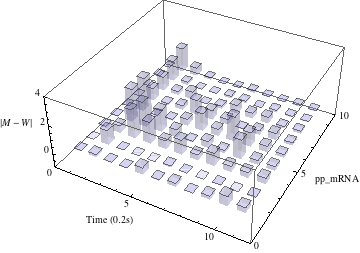
\includegraphics[width=8cm]{tables3f2}
    \caption{График таблицы \ref{m3p2} для $p^*$}
  \end{minipage}
  \hfill
  \begin{minipage}[h]{0.5\linewidth}
    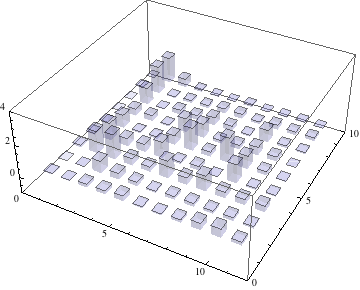
\includegraphics[width=8cm]{tables3f3}
    \caption{График таблицы \ref{m3p3} для $p_{min}$}
  \end{minipage}
\end{figure}

\clearpage
%%%%%%%%%%%%%%%%%%%%%%%%%%%%%%%%%%%%%%%%%%%%%%%%%%%%%%%%%%%%%%%%%%%%%%%%%%%%%%%%
%%%%%%%%%%%%%%%%%%%%%%%%%%%%%%%%%%%%%%%%%%%%%%%%%%%%%%%%%%%%%%%%%%%%%%%%%%%%%%%%
\section{Выводы} \label{s4}

Исходя из численных экспериментов можно сделать несколько выводов:

\begin{enumerate}
  \item Алгоритм ППРЭ хорошо решает поставленную задачу поиска глобального 
  минимума. При этом с биологической точки зрения отличий в поведении системы 
  при использовании найденных параметров нет.
  \item Для данных генных сетей набор параметров обширен, по этой причине 
  существует много вариантов их значений, в которых, возможно, достигается 
  глобальный минимум. Соответственно, если в рамках задачи стоит вопрос поиска 
  конкретного вектора параметров, метод ППРЭ, вероятно, не даст 
  удовлетворительных результатов.
  \item ...
\end{enumerate}

% { \color[HTML]{680100} ЦВЕТНОЙ }

\clearpage
%%%%%%%%%%%%%%%%%%%%%%%%%%%%%%%%%%%%%%%%%%%%%%%%%%%%%%%%%%%%%%%%%%%%%%%%%%%%%%%%
